\chapter{How to train a neural network}
\section{Introduction}
Once we have made our model of a neural network, we would like to train it. The process of training involves tuning the set of weights $W=[w_0,w_1,w_2\hdots]$ associated with each perceptron. To do so we shall give the neural network a rigorous mathematical structure and look at methods to efficiently adjust our weights.
\section{The loss functions}
\begin{marginfigure}
    \begin{center}
        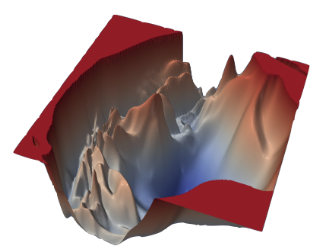
\includegraphics[width=\textwidth]{graphics/resnet110-noskip-loss.png}
    \end{center}
    \caption{A slice of the loss landscape(A graph of $\mathcal L$ vs $(w_i,w_j)$) in ResNet(an example of a type of neural network). Note that it is quite hard to find the minima in this.\citep{li2018visualizing}}
\end{marginfigure}
The loss function can be thought to be a measure of the efficiency of a neural network. Suppose we have a set of observations $ X_0=[X_1,X_2,\hdots X_n]$ with known labels/values $Y_0=[Y_1,Y_2\hdots Y_n]$. Assume our neural network gives predictions $\hat Y_0=[\hat Y_1,\hat Y_2\hdots Y_n]$. Then loss function $\mathcal L(\hat Y_i,Y_i)$ calculates how off our prediction was from the actual label. We define the total loss as $\mathcal L(\hat Y_0,Y_0)=\sum\mathcal L(\hat Y_i,Y_i)$. Generally, we use mean square error(MSE) as the loss function for regression problems and categorical cross entropy for classification problems. That being said, in more complex network, the loss function may be more complicated. For example, a common problem in computer vision is to identify objects in an image. It is found that it is easier to answer the question in two parts:
\begin{enumerate}
    \item Is there an object present in the image?
    \item If yes, where is it in the image?
\end{enumerate}

As we can understand, the first question is a classification problem whereas the second question is a regression problem(assuming we give our answer as coordinates). Now that we have a measure of how good our neural network is, we can think of training to be tuning the parameters to minimise loss.
\section{Gradient Descent}
\begin{marginfigure}
    \begin{center}
        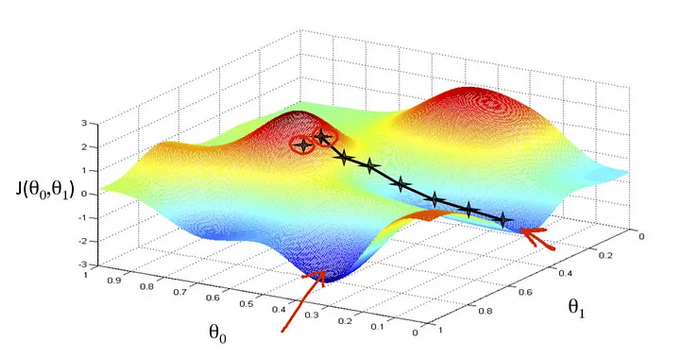
\includegraphics[width=\textwidth]{graphics/grad-desc.png}
    \end{center}
    \caption{Gradient descent, Src: https://towardsdatascience.com/an-intuitive-explanation-
    of-gradient-descent-83adf68c9c33}
\end{marginfigure}
To find the correct set of weights, we use a greedy approach. We check the surrounding landscape
of the weight(i.e. calculate the gradient) and take a step in the direction which leads to maximum
decrease in L. This is an iterative process. Mathematically, for the weight $w_i$ we have the following
update rule:
$$w_i\to w_i-\eta\frac{\partial \mathcal L}{\partial w_i}$$
$\eta$ is known as the learning rate. Fixing $\eta$ is quite tricky: too large and it shoots part the minima, too small and it never converges. The best way to do it is to  use an adaptive learn rate. Some methods(parametric, non-parametric and
hybrid are discussed later, once we cover back propagation)

\section{Neural network as a directed acyclic graph (DAG)}
We look at neural network as a DGA. Each variable (output of perceptron, weight and feature of input) is a vertex. An edge connects vertex $v_i$ to $v_j$ if $v_i$ is directly needed for the computation or updation of $v_j$. For a perceptron with output $x=\sigma\left(w_0+\sum w_ix_i\right)$, there are edges from all $x_i$ and $w_i$ to $x$. In some cases, $\eta$ is not a constant. In that case, there are edges from the parameters $\eta$ depend on to $x$.

\section{Reverse mode auto differentiation}
The general algorithm that is used for gradient descent is called backpropagation. In it's most basic implementation the running time is exponential in the number of layers, which is undesirable. So we talk about a slightly different implementation known as reverse mode auto differentiation$^*$\marginnote{$^*$As it turns out, people in control theory were using this way before this was independently invented for use in deep learning. Kinda shows how low inter topic information sharing is}. Each iteration takes place in two steps: the forward phase and the backward phase. 
\subsection{Forward phase}
In the forward phase, the algorithm simply calculates the total loss $\mathcal L(\hat Y_0,Y_0)$. This is called the forward phase as we calculate along the direction of the edge. 
\subsection{Backward phase}
In that backward phase we calculate the gradients and update weights. We calculate the gradients by repeatedly applying chain rule. If there is an edge from $v_i$ to $v_j$ then $\frac{\partial v_j}{\partial v_i}$ can be calculated directly.  If they don't have an edge connecting them, we take the product of the derivatives  along the edges on a path and then take the sum along all the paths. A small example is given in \ref{chainRule}
\begin{marginfigure}
    \begin{center}
        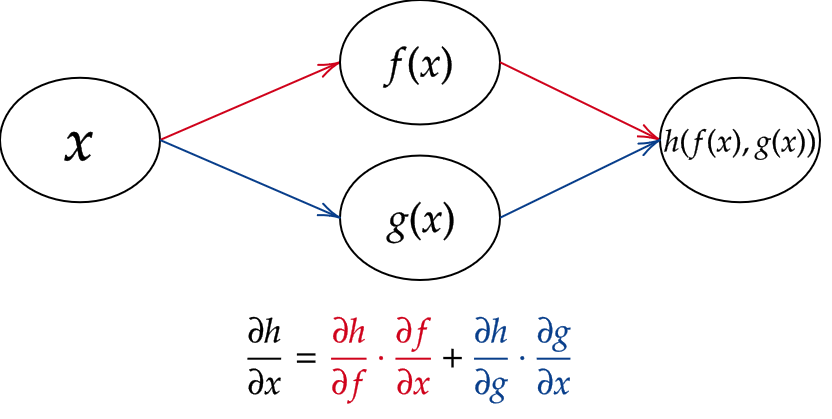
\includegraphics[width=\textwidth]{graphics/chain.png}
    \end{center}
    \caption{A small example of chain rule application}\label{chainRule}
\end{marginfigure}  
At this point it should be obvious that this process is going to take exponentially long the deeper the network is: there are simply too many paths. Here we use dynamic programming. Consider the example in \ref{path}

We see that certain terms are repeated in the expression. This is because parts of the path(shown in colored arrows) is repeated. Therefore, if we can store the gradients for some edges then we don't need to calculate all the terms every time. This significantly reduces computation and makes the algorithm practical to implement. This is called the backward phase as the gradients are calculated against the direction of the edges. 
\section{Gradient Descent Strategies}
\subsection{Stochastic Gradient Descent}
\begin{marginfigure}
    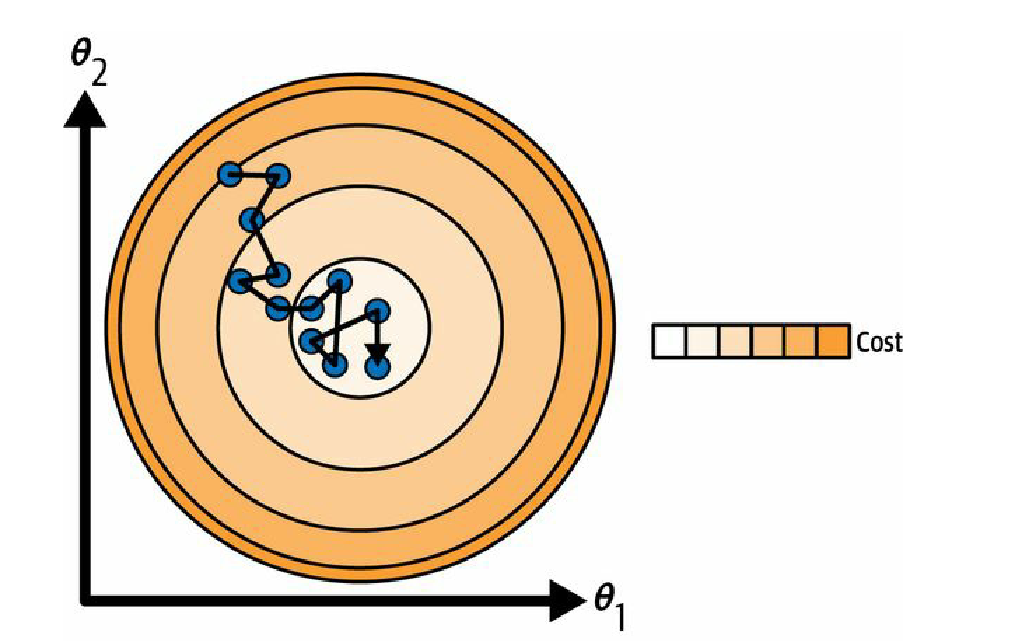
\includegraphics[width=\textwidth]{graphics/stochastic gradient descent.png}
    \caption{Stochastic Gradient Descent. Note that we don't take steps on the best direction, but it is faster.\citep{geron2022hands}}
\end{marginfigure}
Instead of calculating the total loss, we calculate the loss from a randomly picked sample(or a
batch in case of batch gradient descent). Since we are no longer calculating the total loss over all
data points, this decreases the computational time. A proper analogy might be instead of taking
slower but confident steps, we take faster but less-confident steps.
\subsection{Normalization}
\begin{marginfigure}
    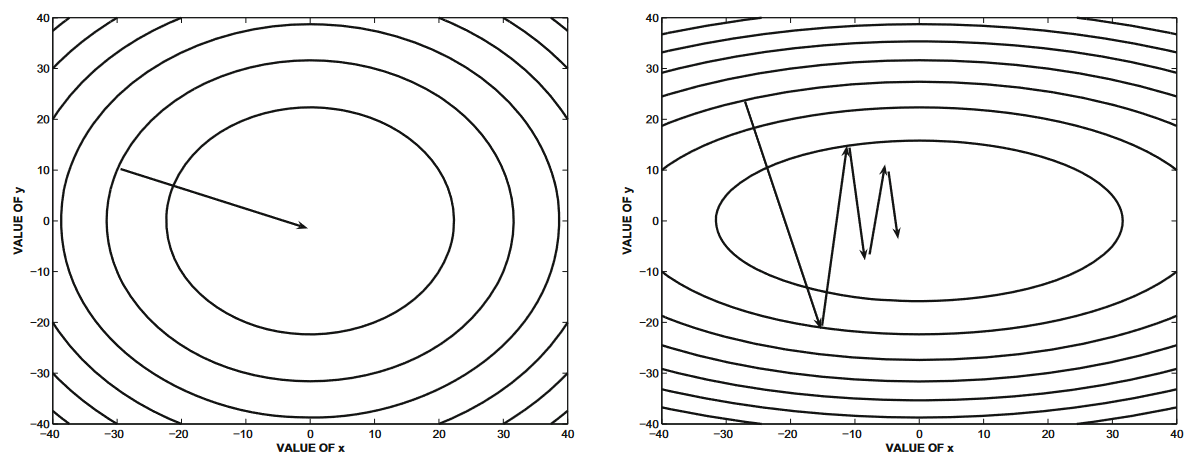
\includegraphics[width=\textwidth]{graphics/normalise.png}
    \caption{Normalization\citep{aggarwal2018neural}}
\end{marginfigure}
Normalizing features is a way to make the descent smoother. It essentially lowers gradient in
directions orthogonal to the minima. This also eases setting the learning rate. If one feature varies between $0$ to 255 and other between 0 and 1, it can be very difficult to set a base learning rate. Normalizing features solves this problem.  
\subsection{Momentum}
\begin{marginfigure}
    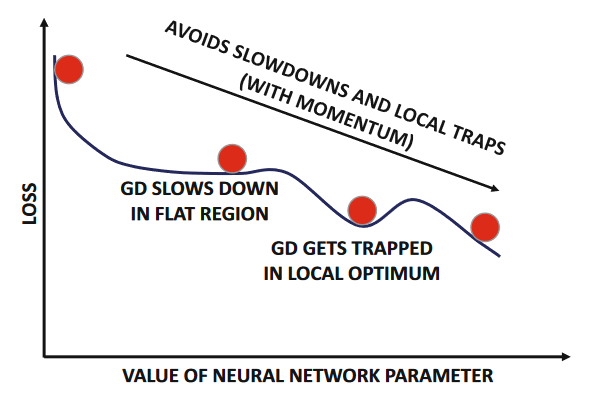
\includegraphics[width=\textwidth]{graphics/momentum.png}
    \caption{Momentum preventing getting stuck at local minima\citep{aggarwal2018neural}}
\end{marginfigure}\begin{marginfigure}
    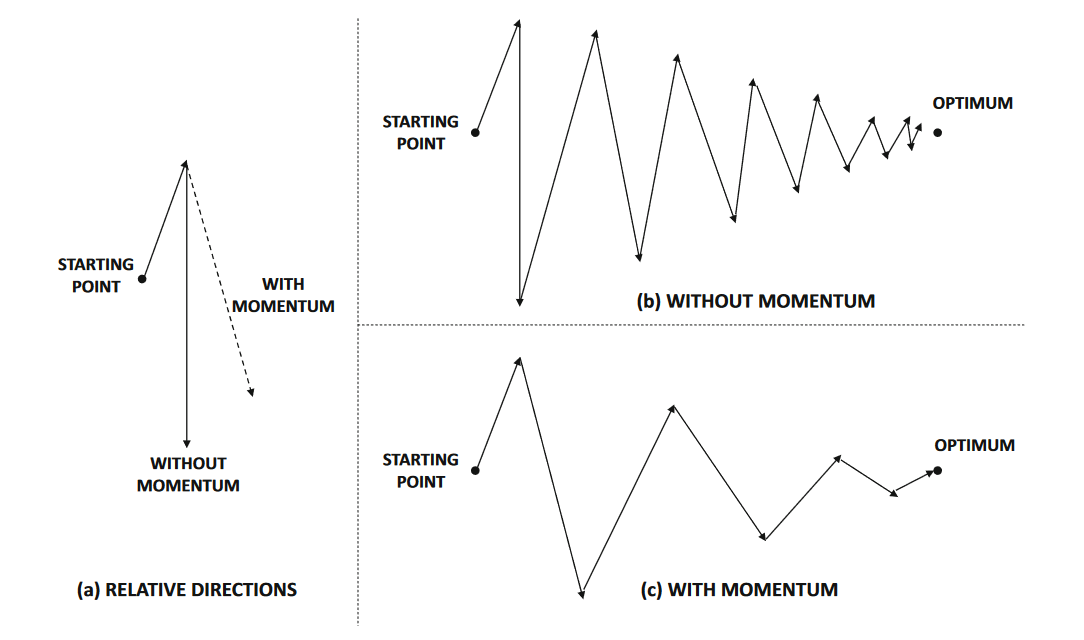
\includegraphics[width=\textwidth]{graphics/momentum-zigzag.png}
    \caption{Momentum reducing zig-zag\citep{aggarwal2018neural}}
\end{marginfigure}
A Momentum term might be used in gradient descent where consideration is made for a moving
average "velocity"  of the descent. Such strategies are particularly helps when there are local
minimas and flat regions. Also helps when there is a lot of ”zig-zag” but the descent on an
average heads in a certain direction. We can improve on this by doing some scout ahead. This
is known as Nestov momentum, and it helps as knowing what's coming up ahead further helps
in correcting the direction of descent.
\begin{figure*}
    \begin{center}
        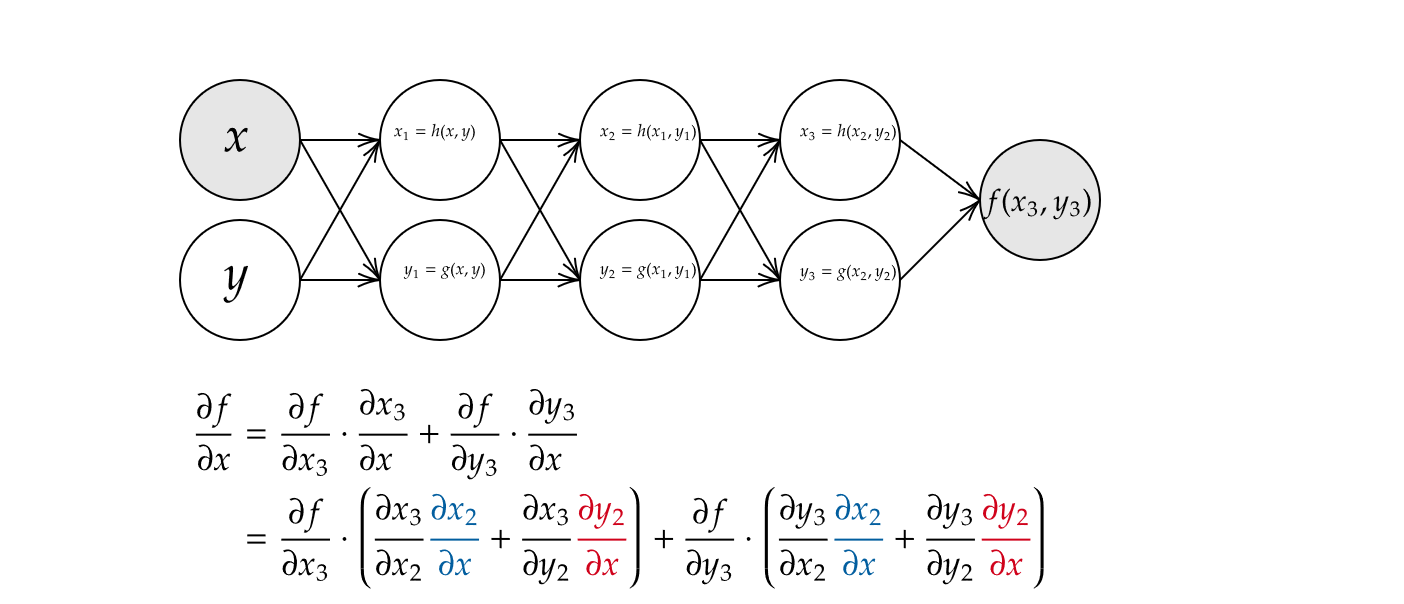
\includegraphics[width=\textwidth]{graphics/revmodeautodiff.png}
        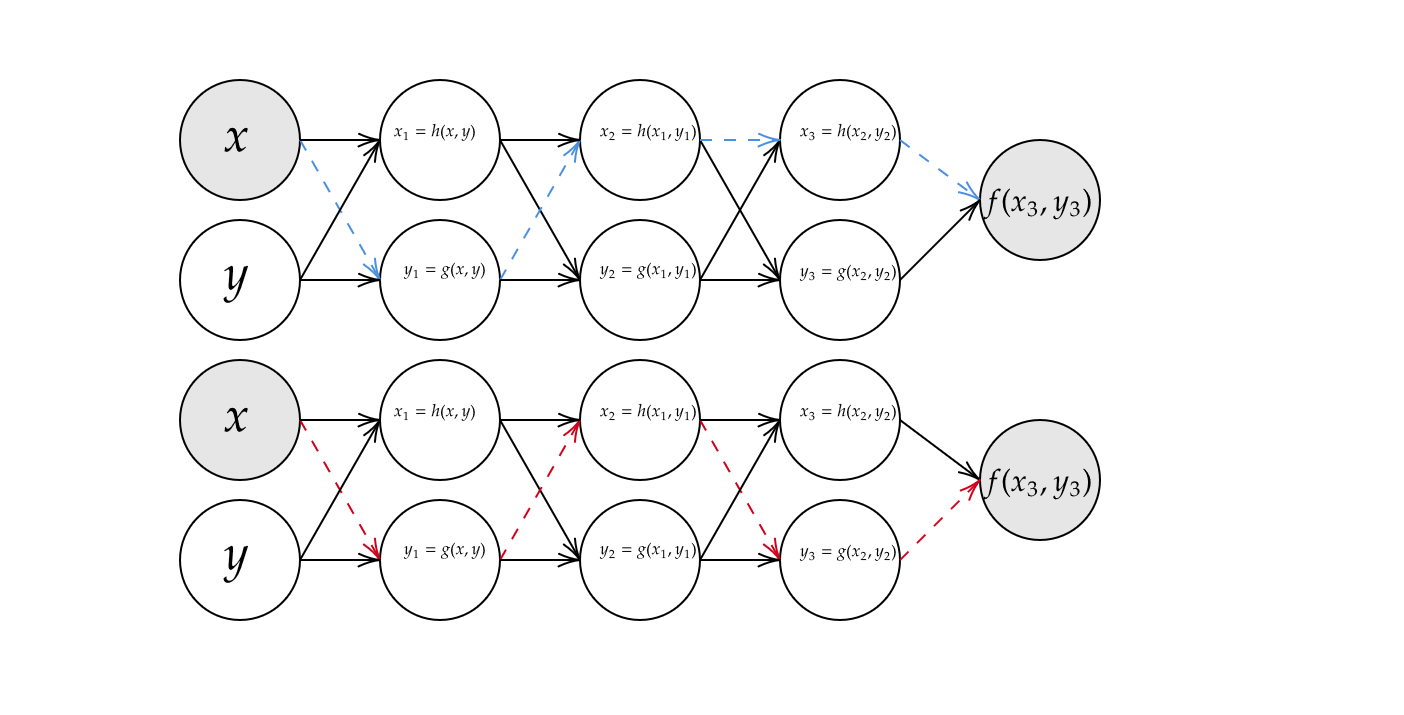
\includegraphics[width=\textwidth]{graphics/path comp.png}
    \end{center}
    \caption{Chain rule in deep networks}\label{path}
\end{figure*}
\section{Setting the learning rate}
\begin{figure}
    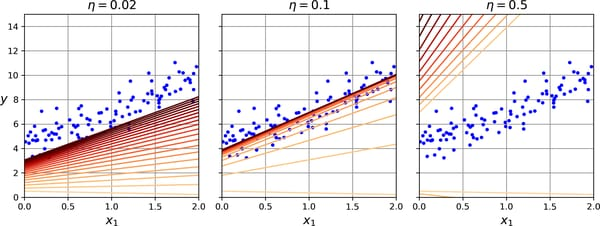
\includegraphics[width=\textwidth]{graphics/learning rate.jpeg}
    \caption{Why is setting a proper learning rate important\citep{geron2022hands}}
\end{figure}
\subsection{Adaptive learning rate}
One way to take care of this problem is  to let different parameters have different learning rates. The idea is that parameters with large partial derivatives are often oscillating
and zigzagging, whereas parameters with small partial derivatives tend to be
more consistent but move in the same direction.
Algorithms include AdaGrad, RMSProp and AdaDelta. Parametric algorithms
combined with momentum considerations also exist: RMSProp with Nesterov
Momentum, ADAM and it's variants like AdaMax, Nadam and AdamW. A quick
comparison table is available at \citep{geron2022hands}
\subsection{Learning rate scheduling}
We have the learning rate high at first so
that it gets a relative idea about where the
minima lies, and then we lower it to find it
with more accuracy. Scheduling is done on numbers of iterations
completed(each iteration is also called an
epoch)
\begin{marginfigure}
    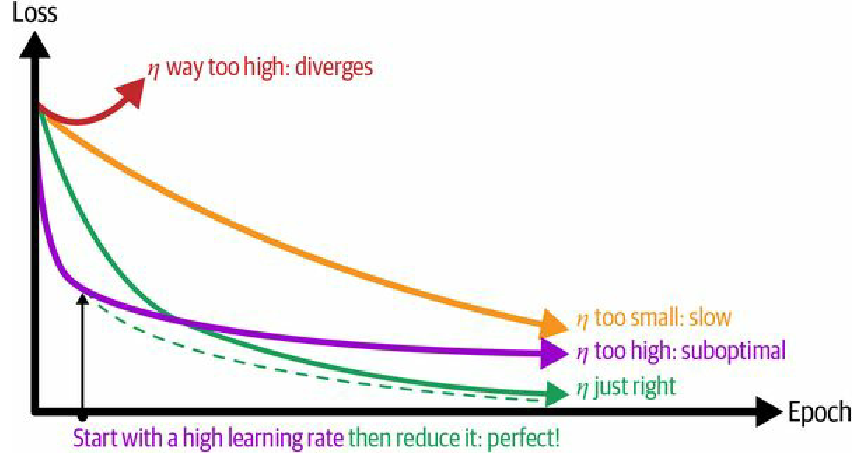
\includegraphics[width=1.3\textwidth]{graphics/learning rate schedule.png}\caption{Learning rate scheduling\citep{geron2022hands}}
\end{marginfigure}
\subsection{One cycle scheduling}
The basic idea behind one cycle scheduling is to start with a low learning
rate, gradually increase it to a maximum value, and then decrease it again to
a low value. This approach helps the network explore a wide range of
learning rates, allowing it to quickly converge to a good solution and
potentially escape from local minima. By using a cyclical learning rate schedule, one cycle scheduling aims to strike
a balance between exploration and exploitation in the learning process. It
enables the network to quickly explore a wide range of learning rates at the
beginning and then gradually refine its weights as the learning rate
decreases.
\section{Choosing Activation function}
The loss function and the gradients propagated backwards depend on the activation functions used. A bad activation function(for example, a function which is not differentiable everywhere) can make training very hard. We first look at some 